\documentclass[10pt]{article}

% ---------- IDIOMA Y CODIFICACIÓN ----------
\usepackage[utf8]{inputenc}
\usepackage[spanish]{babel}
\usepackage{amsmath}
\usepackage[margin=2.5cm]{geometry}
\usepackage{setspace}
\usepackage{graphicx}
\usepackage{tikz}
\usetikzlibrary{circuits.logic.US}

% ---------- TABLAS (Actividad 1: identificación de dispositivos) ----------
\usepackage{booktabs}   % líneas de tabla profesionales (\toprule, \midrule, \bottomrule)
\usepackage{array}
\usepackage{ragged2e}
\usepackage[table]{xcolor} % opcional, para color en encabezado
\usepackage{tabularx}   % columnas que se ajustan al ancho de página
\usepackage{longtable}  % tablas que pueden partirse entre páginas (útil si tu tabla de dispositivos es larga)
\usepackage{caption}    % control de estilo de "Tabla X: ..."
\usepackage{float}
\usepackage{makecell}

% ---------- GLOSARIO (Actividad 2) ----------
% Enfoque simple con "description", sin necesidad de correr makeglossaries aparte
% (evita agregar un paso extra a tu pipeline de compilación).
\usepackage{enumitem}
\newlist{glosario}{description}{1}
\setlist[glosario]{
    font=\normalfont\bfseries,
    leftmargin=0pt,
    labelsep=0.5em,
    itemsep=0.5em
}

% ------- TABLAS PARA EMULADOR 8086 ---
% Uso dentro del documento:
%   \begin{glosario}
%       \item[Chipset] Definición y características...
%   \end{glosario}

% ---------- PLACEHOLDER \relleno ----------
% Uso: \relleno              -> texto de aviso genérico
%      \relleno{Tu texto}    -> muestra tu texto en rojo (útil para ir dejando borradores)
\newcommand{\relleno}[1][\textbf{[COMPLETAR AQUÍ]}]{\textcolor{red}{#1}}
% ---------- CONFIGURACIONES PARA ENCABEZADO Y PORTADA ----------
\usepackage{colortbl}
\usepackage[colorlinks=true,linkcolor=black,urlcolor=black,citecolor=black]{hyperref}

% Definición de colores y columnas personalizadas (usadas en la portada)
\definecolor{tablebackground}{rgb}{0.8, 0, 0}
\newcolumntype{x}[1]{>{\centering\arraybackslash\hspace{0pt}}p{#1}}
\newcolumntype{M}[1]{>{\centering\arraybackslash}m{#1}}
\newcolumntype{N}{@{}m{0pt}@{}}
\newcolumntype{P}[1]{>{\RaggedRight\arraybackslash}p{#1}}

% Variables de datos para la portada y encabezado
\newcommand{\itemEmail}{ccapatinta@unsa.edu.pe}
\newcommand{\itemStudent}{Camilo B.A. Capatinta Almanza (Teoría grupo B)}
\newcommand{\itemCourse}{Lab. Arq. de computadoras}
\newcommand{\itemCourseCode}{1702227}
\newcommand{\itemSemester}{IV}
\newcommand{\itemUniversity}{Universidad Nacional de San Agustín de Arequipa}
\newcommand{\itemFaculty}{Facultad de Ingeniería de Producción y Servicios}
\newcommand{\itemDepartment}{Departamento Académico de Ingeniería de Sistemas e Informática}
\newcommand{\itemSchool}{Escuela Profesional de Ingeniería de Sistemas}
\newcommand{\itemAcademic}{2026 - B}
\newcommand{\itemInput}{29/09/2026}
\newcommand{\itemOutput}{--/10/2026}
\newcommand{\itemPracticeNumber}{03}
\newcommand{\itemTheme}{Programación para el microprocesador INTEL - Instrucciones de transferencia de datos}

% Configuración del encabezado y pie de página (fancyhdr)
\usepackage{fancyhdr}
\pagestyle{fancy}
\fancyhf{}
\setlength{\headheight}{40.51407pt}
\renewcommand{\headrulewidth}{1pt}
\renewcommand{\footrulewidth}{1pt}

% Encabezado
\fancyhead[L]{\raisebox{-0.2\height}{
\includegraphics[width=3cm]{img/logo_episunsa.png}}}
\fancyhead[C]{\fontsize{7}{7}\selectfont    \itemUniversity \\ \itemFaculty \\ \itemDepartment \\ \itemSchool \\ \textbf{\itemCourse}}
\fancyhead[R]{\raisebox{-0.2\height}{
\includegraphics[width=1.2cm]{img/logo_abet.png}}}

% Pie de página
\fancyfoot[L]{Estudiante Camilo Capatinta}
\fancyfoot[C]{\itemCourse}
\fancyfoot[R]{Página \thepage}

\begin{document}

% --- INICIO DE LA PORTADA ---
	\vspace*{10px}
	
	\begin{center}
		\parbox{0.8\textwidth}{\centering\fontsize{17}{20}\selectfont\textbf{Informe de laboratorio \itemPracticeNumber}}
	\end{center}
	\begin{center}
		\parbox{0.8\textwidth}{\centering\textbf{\Large Tema: \itemTheme}}
	\end{center}

\begin{flushright}
    \begin{tabular}{|M{2.5cm}|N|}
        \hline 
        \rowcolor{tablebackground}
        \color{white} \textbf{Nota}  \\
        \hline 
             \\[30pt]
        \hline          
    \end{tabular}
\end{flushright}    

\begin{table}[h!]
    \begin{tabular}{|x{4.7cm}|x{4.8cm}|x{4.8cm}|}        
        \hline 
        \rowcolor{tablebackground}
        \color{white} \textbf{Estudiante} & \color{white}\textbf{Escuela}  & \color{white}\textbf{Asignatura}   \\
        \hline 
        {\itemStudent \par \itemEmail} & \itemSchool & {\itemCourse \par Semestre: \itemSemester \par Código: \itemCourseCode}     \\
        \hline          
    \end{tabular}
\end{table}     

\begin{table}[H]
    \begin{tabular}{|x{4.7cm}|x{4.8cm}|x{4.8cm}|}
        \hline 
        \rowcolor{tablebackground}
        \color{white}\textbf{Laboratorio} & \color{white}\textbf{Tema}  & \color{white}\textbf{Duración}   \\
        \hline 
        \itemPracticeNumber & \itemTheme & 02 horas   \\
        \hline 
    \end{tabular}
\end{table}

\begin{table}[H]
    \begin{tabular}{|x{4.7cm}|x{4.8cm}|x{4.8cm}|}
        \hline 
        \rowcolor{tablebackground}
        \color{white}\textbf{Semestre académico} & \color{white}\textbf{Fecha de inicio}  & \color{white}\textbf{Fecha de entrega}   \\
        \hline 
        \itemAcademic & \itemInput &  \itemOutput  \\
        \hline 
    \end{tabular}
\end{table}

\newpage
\tableofcontents
\thispagestyle{plain}
\clearpage

% --- FIN DE LA PORTADA ---

% ============================================================
% Sección: Actividades
% Diseño e implementación de un sumador total de un bit
% Simulador de Circuitos Digitales 0.9.5 (tourdigital.net)
% ============================================================
\section{Actividades}
\subsection{Programa 1: Instrucciones de transferencia de datos}

Ahora analice el siguiente código fuente (llamado PRIMER PROGRAMA),
ayudándose de los comentarios y del diagrama de flujo que lo acompaña. Intente
predecir cada cambio que tendrán los datos hexadecimales en los registros del
microprocesador.

\begin{figure}[H]
    \centering
    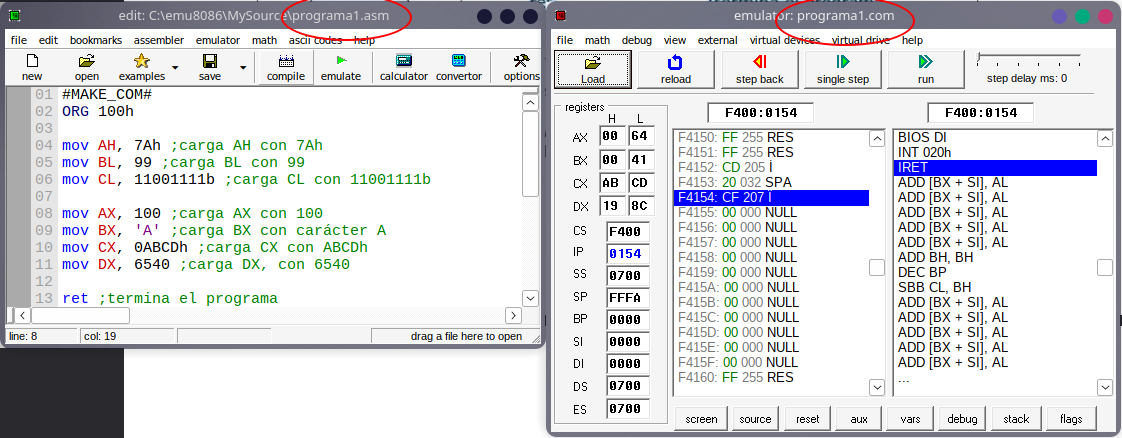
\includegraphics[width=0.8\textwidth]{img/1.png}
    \caption{programa1.asm}
    \label{fig:programa1.asm}
\end{figure}

\begin{itemize}
    \item Observe que el sistema le asigna al archivo .COM el mismo nombre que el archivo .asm, es decir, programa1.com
\end{itemize}

\begin{figure}[H]
    \centering
    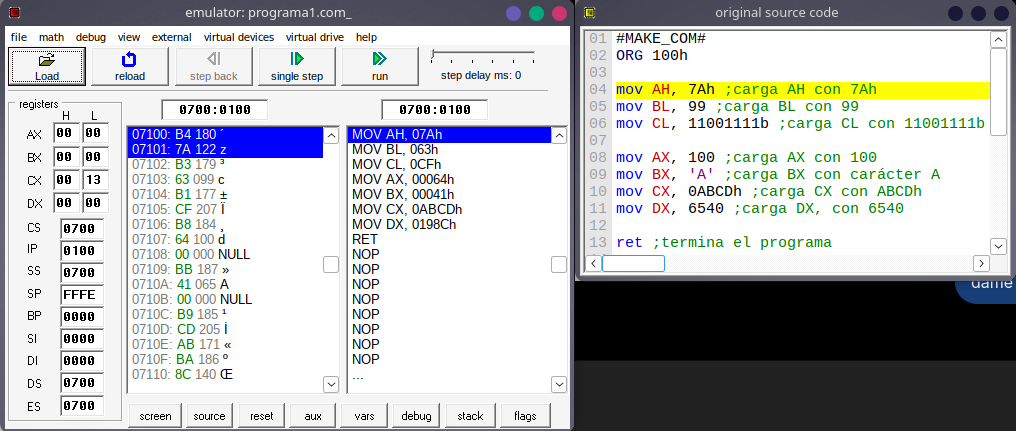
\includegraphics[width=0.8\textwidth]{img/2.png}
    \caption{Emulador de programa1.asm}
    \label{fig:emulador_programa1_antes}
\end{figure}

\begin{itemize}
    \item Copie los datos almacenados en los registros antes de ejecutar el programa:
\end{itemize}
% Tabla 12
\begin{table}[H]
\centering
\begin{tabular}{|c|c|c|c|}
\hline
AX: 0000 & BX: 0000 & CX: 0000 & DX: 0000 \\ \hline
CS: 0700 & DS: 0700 & ES: 0700 & SS: 0700 \\ \hline
BP: 0000 & IP: 0100 & SP: FFFE& \cellcolor{gray!40} \\ \hline
DI: 0000 & SI: 0000 & \cellcolor{gray!40} & \cellcolor{gray!40} \\ \hline
\end{tabular}
\caption{Datos almacenados antes de ejecutar el programa.}
\end{table}

\begin{itemize}
    \item Ejecute el programa totalmente (RUN) y anote los datos resultantes. Verifique
si concuerdan con los datos que usted esperaba.
\end{itemize}

\begin{figure}[H]
    \centering
    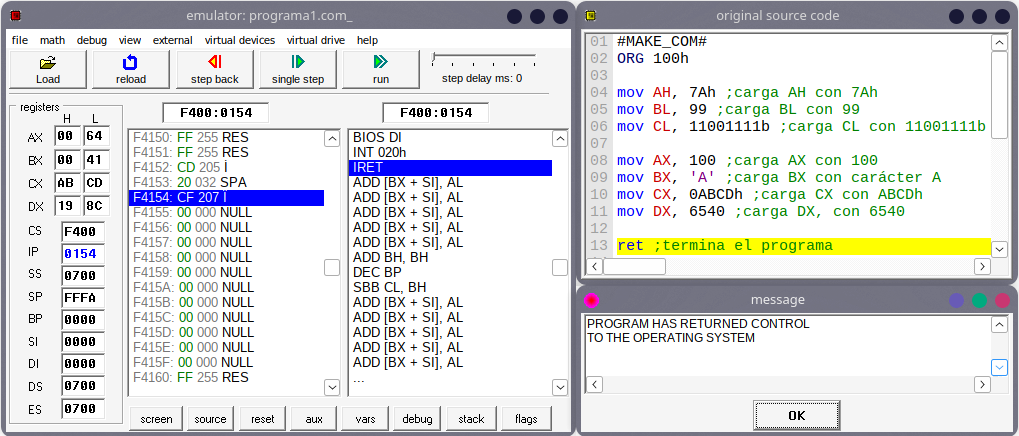
\includegraphics[width=0.8\textwidth]{img/3.png}
    \caption{Emulador de programa1.asm}
    \label{fig:emulador_programa1_resultante}
\end{figure}
% Tabla 13
\begin{table}[H]
\centering
\begin{tabular}{|c|c|c|c|}
\hline
AX: 0064 & BX: 0041 & CX: ABCD & DX: 198C \\ \hline
CS: F400 & DS: 0700 & ES: 0700 & SS: 0700 \\ \hline
BP: 0000 & IP: 0154 & SP: FFFA & \cellcolor{gray!40} \\ \hline
DI: 0000 & SI: 0000 & \cellcolor{gray!40} & \cellcolor{gray!40} \\ \hline
\end{tabular}
\caption{Datos resultantes después de ejecutar el programa.}
\end{table}

\begin{itemize}
    \item Ejecute el emulador con Single step y anote los resultados en la Cuadro.
\end{itemize}

\begin{figure}[H]
    \centering
    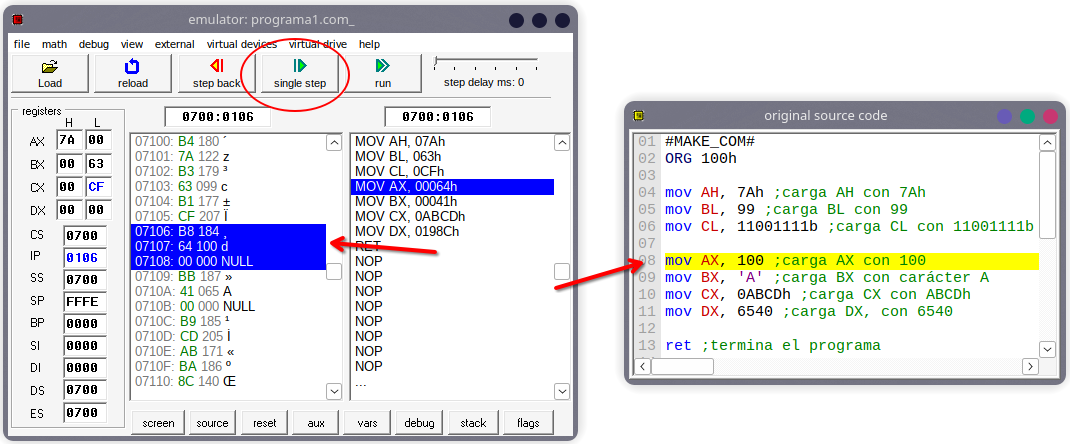
\includegraphics[width=0.8\textwidth]{img/4.png}
    \caption{Emulador ejecutado con Single step}
    \label{fig:emulador_Single_step}
\end{figure}

% Preámbulo: \usepackage{array,tabularx,makecell}

\begin{table}[H]
\centering
\caption{Programa 1: transferencia de datos}
\renewcommand{\arraystretch}{1.2}
\setlength{\tabcolsep}{4pt}
\begin{tabularx}{\textwidth}{|>{\centering\arraybackslash}p{0.10\textwidth}|>{\centering\arraybackslash}p{0.10\textwidth}|>{\centering\arraybackslash}p{0.07\textwidth}|>{\centering\arraybackslash}p{0.07\textwidth}|>{\centering\arraybackslash}p{0.07\textwidth}|>{\centering\arraybackslash}X|}
\hline
\multicolumn{2}{|c|}{\textbf{DIRECCIONES}} &
\multicolumn{3}{c|}{\makecell{\textbf{LENGUAJE DE}\\\textbf{MÁQUINA}}} &
\makecell{\textbf{LENGUAJE}\\\textbf{ENSAMBLADOR}} \\ \hline

\textbf{SEGM (CS)} & \textbf{OFFSET} &
\multicolumn{3}{c|}{\textbf{CAMPOS}} &
\textbf{LÍNEA} \\ \hline

0700 & 0100 & B4 & 7A &    & mov AH, 7Ah \\ \hline
0700 & 0102 & B3 & 63 &    & mov BL, 99 \\ \hline
0700 & 0104 & B1 & CF &    & mov CL, 11001111b \\ \hline
0700 & 0106 & B8 & 64 & 00 & mov AX, 100 \\ \hline
0700 & 0109 & BB & 41 & 00 & mov BX, 78 \\ \hline
0700 & 010C & B9 & CD & AB & mov CX, 0ABCDh \\ \hline
0700 & 010F & BA & 8C & 19 & mov DX, 6540 \\ \hline
0700 & 0112 & C3 &    &    & ret \\ \hline

\multicolumn{6}{|c|}{\makecell{\textbf{NOTA: A partir de este punto el programa ejecuta un procedimiento}\\
\textbf{predeterminado llamado Interrupción.}}} \\ \hline

0700 & 0000 & CD & 20 &    & INT 20h \\ \hline
F400 & 0150 & FF & FF &    & BIOS DI \\ \hline
\end{tabularx}
\end{table}

\subsection{Programa 2: Modos de direccionamiento con MOV}
¿Cómo el ensamblador se traduce a lenguaje máquina (opcodes, direcciones, tamaño de cada instrucción) y cómo el IP avanza por el programa?

% Preámbulo: \usepackage{array,tabularx,makecell}

\begin{table}[H]
\centering
\caption{Registros antes y después de cada instrucción}
\renewcommand{\arraystretch}{1.5}
\setlength{\tabcolsep}{4pt}
\begin{tabularx}{\textwidth}{|>{\centering\arraybackslash}p{0.11\textwidth}|>{\centering\arraybackslash}p{0.11\textwidth}|>{\centering\arraybackslash}X|>{\centering\arraybackslash}X|>{\centering\arraybackslash}X|>{\centering\arraybackslash}X|>{\centering\arraybackslash}X|}
\hline
\makecell{\textbf{Reg.Seg}\\\textbf{(DS)}} &
\makecell{\textbf{OFFSET}\\\textbf{(IP)}} &
\makecell{\textbf{Inicio del}\\\textbf{programa}} &
\textbf{Antes de 5\textordfeminine} &
\textbf{Después de 5\textordfeminine} &
\textbf{Después de 6\textordfeminine} &
\textbf{Después de 7\textordfeminine} \\ \hline

0700 & \textbf{0112h} & 90 & 90 & 61 & 61 & 61 \\ \hline
0700 & \textbf{0113h} & 90 & 90 & 90 & 41 & 41 \\ \hline
\multicolumn{2}{|c|}{\textbf{REGISTRO CX}} & 0011 & 0011 & 0011 & 4161 & 4161\\ \hline
\end{tabularx}
\end{table}

%-- IMAGENES DEL REGISTRO DE TABLA 4
\begin{figure}[H]
    \centering
    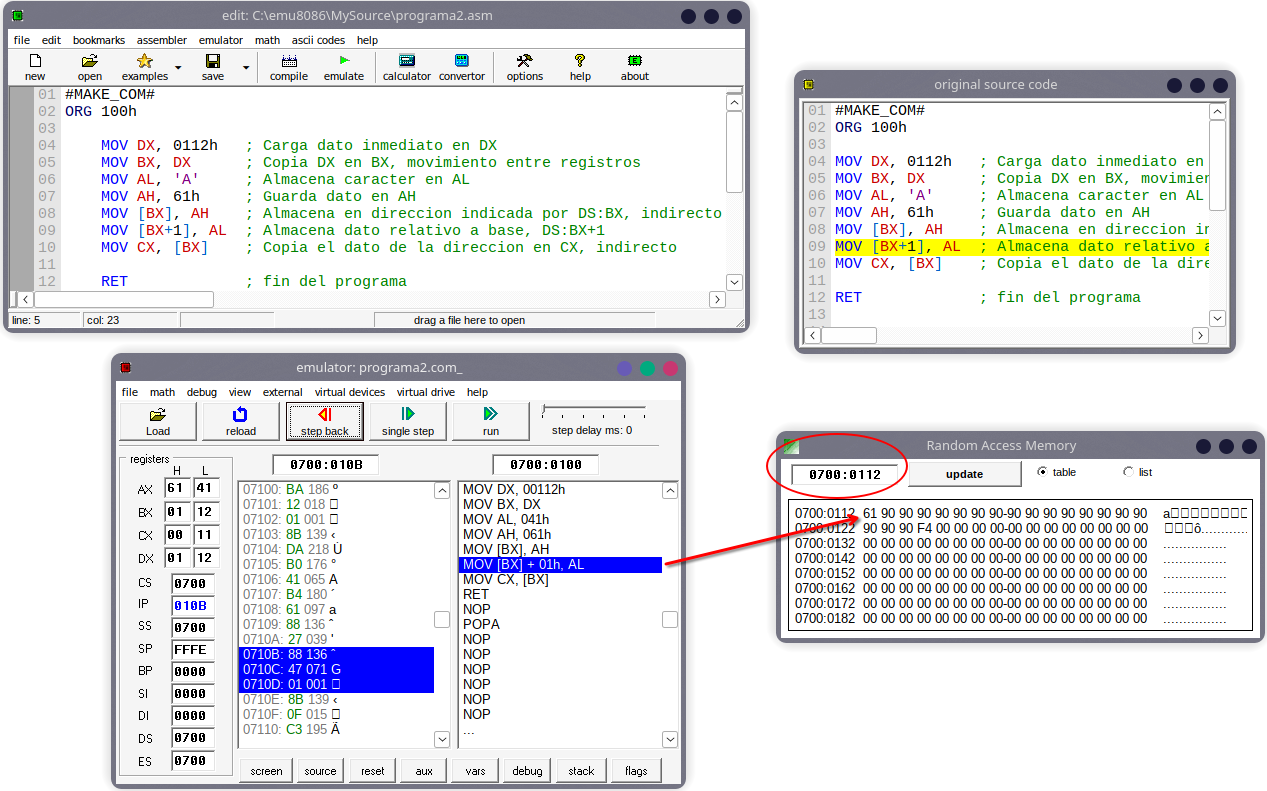
\includegraphics[width=0.8\textwidth]{img/5.png}
    \caption{Visualización de cambio de registros y de direcciones de memoria usando Single step}
    \label{fig:cambio_direcciones}
\end{figure}
% Preámbulo: \usepackage{array,tabularx,makecell}

\begin{table}[H]
\centering
\caption{Direcciones, lenguaje de máquina y lenguaje ensamblador}
\renewcommand{\arraystretch}{1.8}
\setlength{\tabcolsep}{4pt}
\begin{tabularx}{\textwidth}{|>{\centering\arraybackslash}p{0.10\textwidth}|>{\centering\arraybackslash}p{0.10\textwidth}|>{\centering\arraybackslash}p{0.07\textwidth}|>{\centering\arraybackslash}p{0.07\textwidth}|>{\centering\arraybackslash}p{0.07\textwidth}|>{\centering\arraybackslash}X|}
\hline
\multicolumn{2}{|c|}{\textbf{DIRECCIONES}} &
\multicolumn{3}{c|}{\textbf{LENGUAJE DE MÁQUINA}} &
\textbf{LENGUAJE ENSAMBLADOR} \\ \hline

\textbf{SEGM (CS)} & \textbf{OFFSET} &
\multicolumn{3}{c|}{\textbf{CAMPOS}} &
\textbf{LÍNEA} \\ \hline

 0700 & 0100 & BA & 12 & 01 & MOV DX, 0112h \\ \hline
 0700 & 0103 & 8B & DA &  & MOV BX, DX \\ \hline
 0700 & 0105 & B0 & 41 &  & MOV AL, 'A' \\ \hline
 0700 & 0107 & B4 & 61 &  & MOV AH, 61h \\ \hline
 0700 & 0109 & 88 & 27 &  & MOV [BX], AH \\ \hline
 0700 & 010B & 88 & 47 & 01 & MOV [BX+1], AL \\ \hline
 0700 & 010E & 8B & 0F &  & MOV CX, [BX] \\ \hline
 0700 & 0110 & C3 &  &  & RET \\ \hline
\end{tabularx}
\end{table}

\subsection{Programa 3: Escritura directa en memoria de video}

Escribir directamente en la memoria de video (segmento B800h) para imprimir un carácter con color de fondo y de letra, y entender el byte de atributo.

\begin{figure}[H]
    \centering
    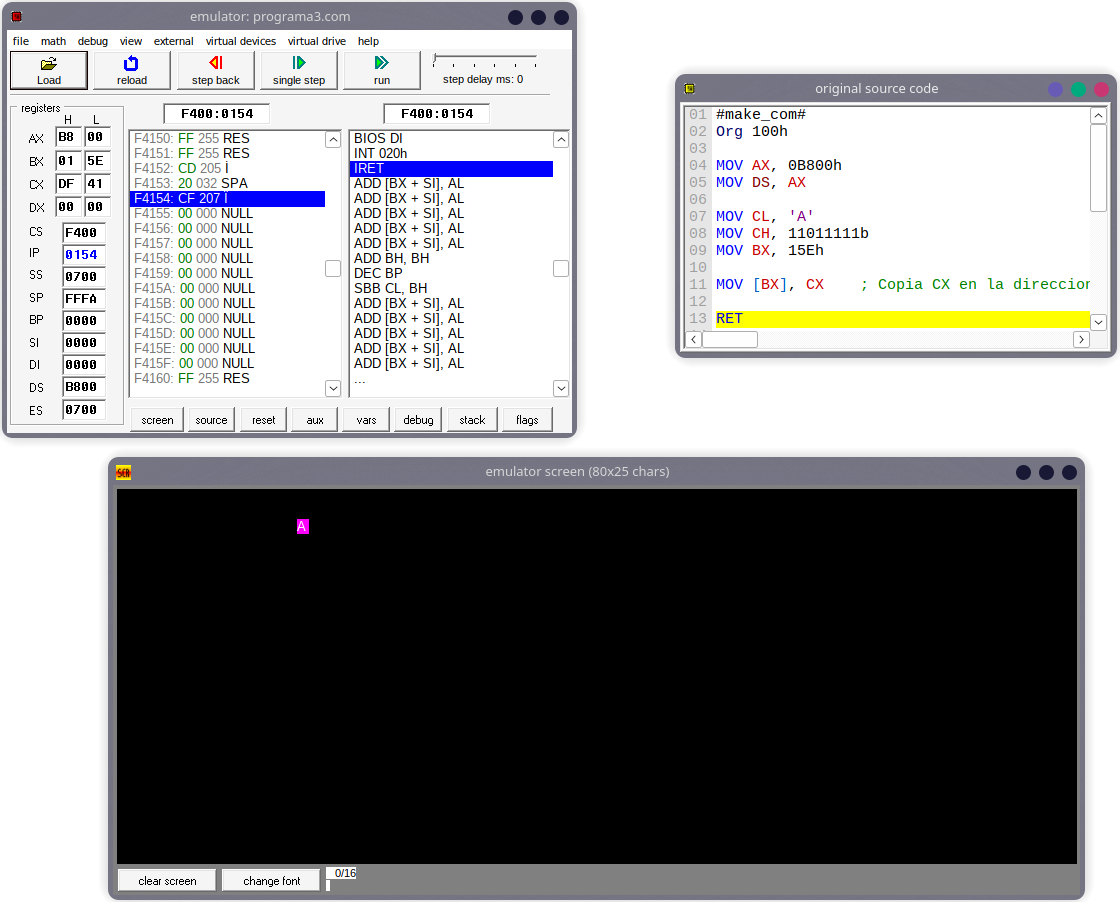
\includegraphics[width=0.8\textwidth]{img/6.png}
    \caption{Emulación de programa3.asm}
    \label{fig:programa3.asm}
\end{figure}

\begin{itemize}
    \item \textbf{Observación:} El programa imprime el caracter 'A' de color blanco y fondo fucsia, ubicado en la 3ra fila y columna 16.
\end{itemize}

\begin{figure}[H]
    \centering
    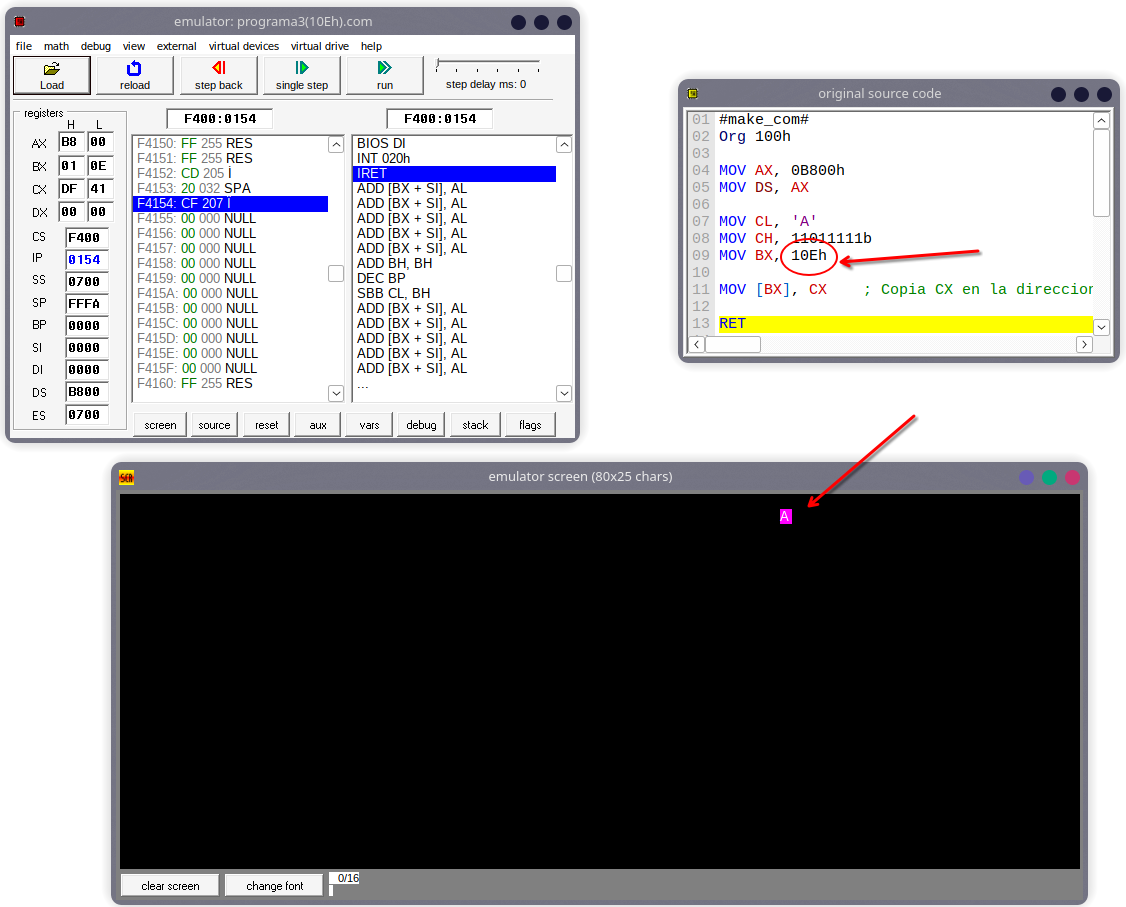
\includegraphics[width=0.8\textwidth]{img/7.png}
    \caption{Emulación de programa3(10Eh).asm}
    \label{fig:programa3(10Eh).asm}
\end{figure}

\begin{itemize}
    \item \textbf{Observación:} A diferencia del anterior, este cambia de ubicación al caracter, poniéndolo en la 2da fila y columna 56.
\end{itemize}

 \begin{figure}[H]
    \centering
    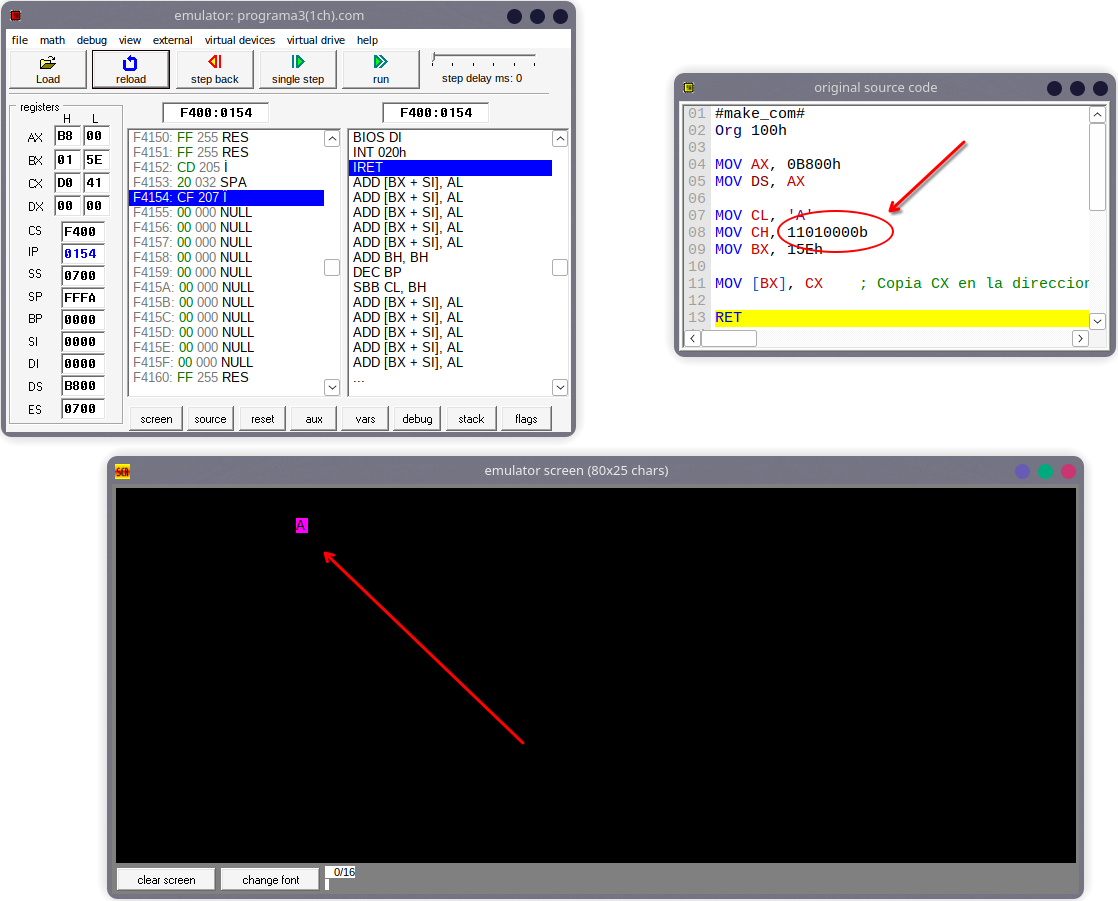
\includegraphics[width=0.8\textwidth]{img/8.png}
    \caption{Emulación de programa3(1ch).asm: CH cambiado a 11010000b}
    \label{fig:programa3(1ch).asm}
\end{figure}

\begin{itemize}
    \item \textbf{Observación:} En este caso, el programa cambia solo el color del caracter (negro). Esto lo hace cambiando el valor de CH a 11010000b.
\end{itemize}

 \begin{figure}[H]
    \centering
    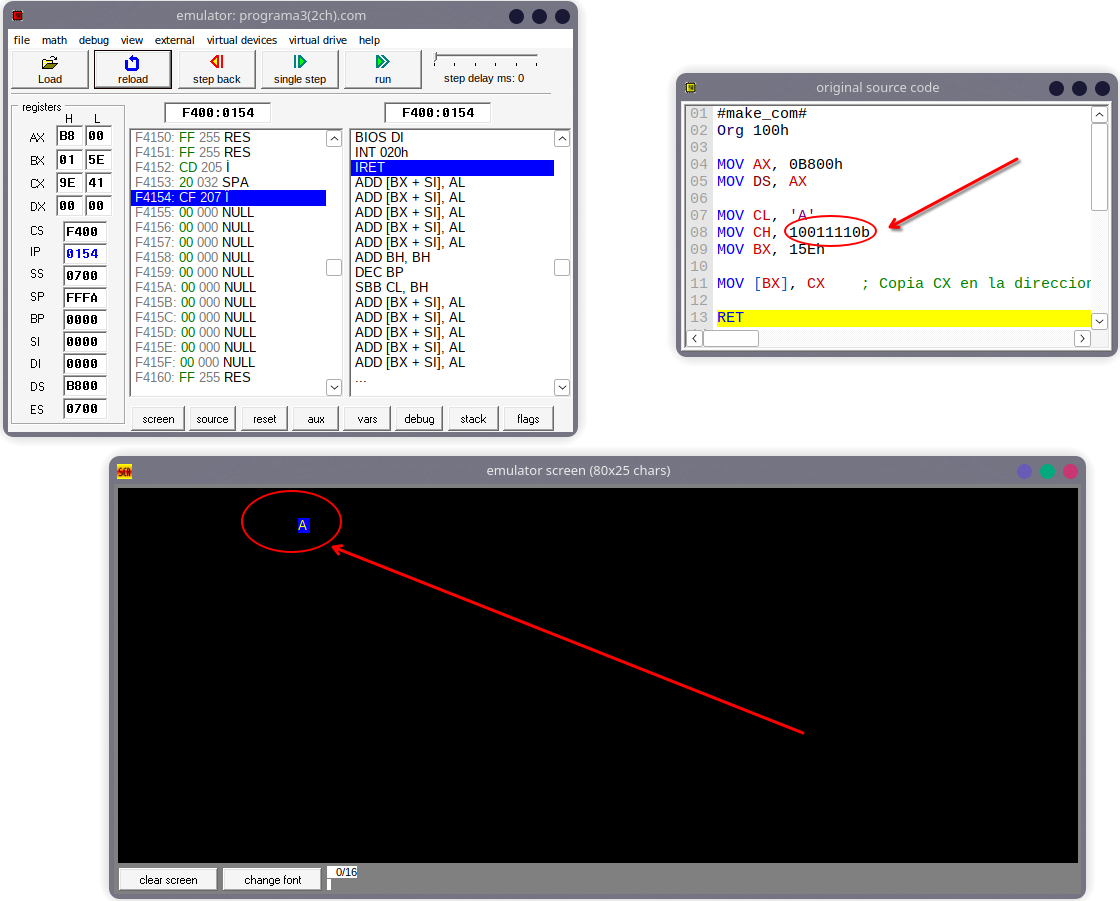
\includegraphics[width=0.8\textwidth]{img/9.png}
    \caption{Emulación de programa3(2ch).asm: CH cambiado a 10011110b}
    \label{fig:programa3(2ch).asm}
\end{figure}

\begin{itemize}
    \item \textbf{Observación:} En este caso, el programa cambia el color del fondo del caracter (amarillo) y del caracter mismo(azul claro). Esto lo hace cambiando el valor de CH a 10011110b.
\end{itemize}

 \begin{figure}[H]
    \centering
    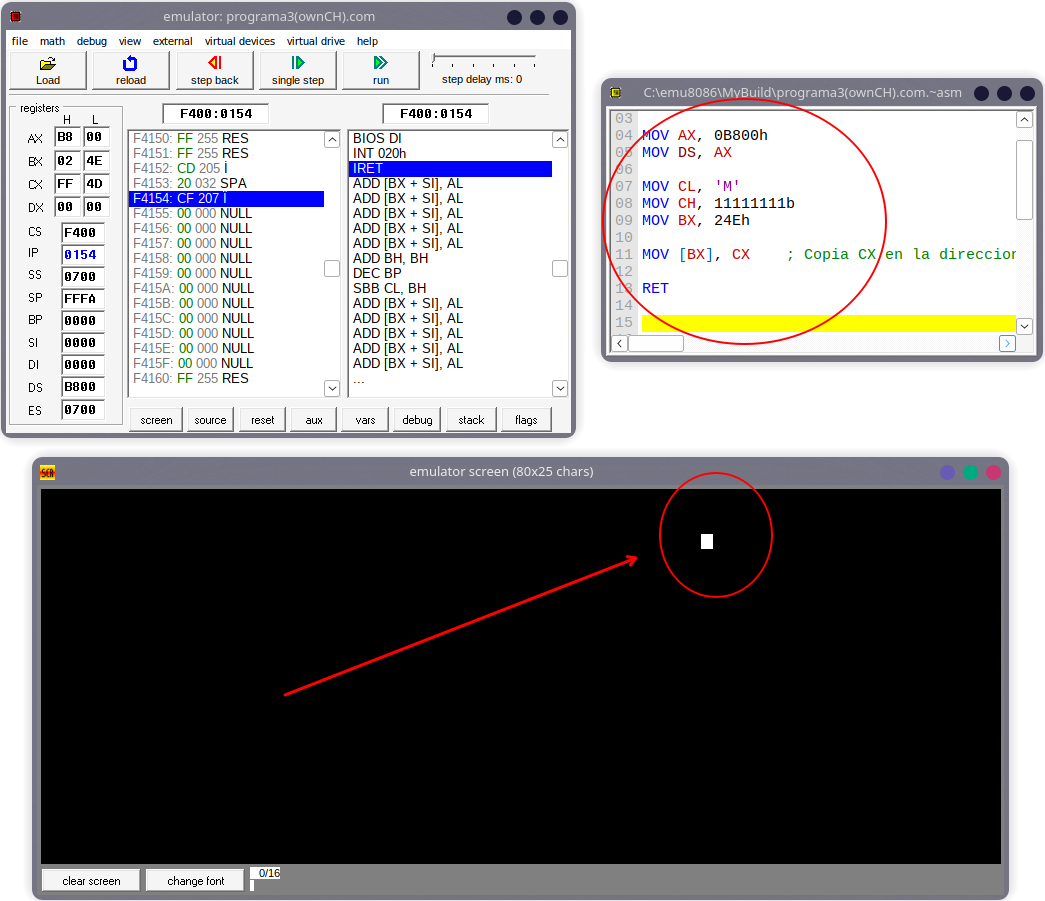
\includegraphics[width=0.8\textwidth]{img/10.png}
    \caption{Emulación de programa3(ownCH).asm: CL = 'M', CH = 11111111b, BX = 24Eh}
    \label{fig:programa3(ownCH).asm}
\end{figure}

\begin{itemize}
    \item \textbf{Observación:} Para este programa se ha cambiado los 3 valores de CL, CH y BX. Los cambios respectivos son: Ahora el caracter es 'M', CH = 11111111h, es decir, fondo y color del caracter blancos, BX = 24Eh, es decir, el caracter se encuentra en la 4ta fila y en la columna 56.
\end{itemize}


\section{Cuestionario}

\begin{enumerate}
  \renewcommand{\labelenumi}{\alph{enumi})}
  \renewcommand{\labelenumii}{\arabic{enumii}.}

  \item \textbf{Primer programa.}
  \begin{enumerate}
    \item \textbf{En el encabezado del programa, ¿por qué se incluye la línea \texttt{org 100h}?}\\
    Porque un archivo \texttt{.COM} se carga en memoria dejando libres los primeros 256 bytes (100h) del segmento para el PSP (\textit{Program Segment Prefix}). El código comienza entonces en el desplazamiento 0100h. La directiva \texttt{ORG} le indica al ensamblador que calcule todas las direcciones a partir de ese punto, y por eso al cargar el programa IP vale 0100.

    \item \textbf{Al introducir datos en los registros se usan diferentes formatos (bases de numeración), ¿cuántos y cuáles son?}\\
    Se usaron cuatro formatos: decimal (\texttt{99}, \texttt{100}, \texttt{6540}), hexadecimal (\texttt{7Ah}, \texttt{0ABCDh}), binario (\texttt{11001111b}) y carácter ASCII (\texttt{'A'}). En los tres primeros la base se indica con el sufijo (ninguno, \texttt{h} o \texttt{b}), y el carácter entre comillas se convierte a su código ASCII (41h).

    \item \textbf{La sintaxis de MOV define tres campos: instrucción, dato1 y dato2. Al moverse los datos, ¿cuál es la fuente y cuál el destino?}\\
    El formato es \texttt{MOV destino, fuente}: \textit{dato1} es el destino y \textit{dato2} es la fuente. Por ejemplo, en \texttt{MOV AH, 7Ah} el destino es AH y la fuente es el valor 7Ah. El dato se copia, por lo que la fuente no se modifica.

    \item \textbf{Al observar la Tabla 1 se nota que a la misma instrucción MOV se le asignan diferentes códigos hexadecimales, ¿a qué se debe esto?}\\
    El código de operación depende del registro destino y del tamaño del operando. Para cargar un dato inmediato en un registro de 8 bits el código es B0h más el número del registro (B4 para AH, B3 para BL, B1 para CL). Para registros de 16 bits es B8h más el número del registro (B8 para AX, BB para BX, B9 para CX, BA para DX). Es decir, aunque el mnemónico sea el mismo, el procesador necesita un código distinto para cada combinación.

    \item \textbf{¿Cuál es la función que cumple el registro IP dentro del primer programa?}\\
    IP (\textit{Instruction Pointer}) contiene el desplazamiento, dentro del segmento de código CS, de la siguiente instrucción por ejecutar. La pareja CS:IP indica al procesador dónde leer. Comienza en 0100h y se incrementa automáticamente según el tamaño de cada instrucción ejecutada, avanzando por el programa hasta llegar a \texttt{RET}.

    \item \textbf{En la columna OFFSET de la Tabla 1 los valores no se incrementan a una razón constante, ¿por qué?}\\
    Porque las instrucciones no ocupan el mismo número de bytes. Las instrucciones con dato inmediato de 8 bits (por ejemplo \texttt{MOV AH, 7Ah}) miden 2 bytes, las de 16 bits (por ejemplo \texttt{MOV AX, 100}) miden 3 bytes y \texttt{RET} mide 1 byte. Cada offset es el anterior más el tamaño de esa instrucción: 0100, 0102, 0104, 0106, 0109, 010C, 010F y 0112.
  \end{enumerate}

  \item \textbf{Segundo programa.}
  \begin{enumerate}
    \item \textbf{Al comparar las dos primeras instrucciones, ¿qué diferencias hay al ejecutarlas, siendo que las dos son MOV?}\\
    \texttt{MOV DX, 0112h} usa direccionamiento inmediato: el dato forma parte de la propia instrucción (3 bytes: BA 12 01) y se carga en DX. \texttt{MOV BX, DX} usa direccionamiento por registro: copia el contenido de un registro en otro, no lleva dato inmediato y ocupa solo 2 bytes (8B DA). En ambas solo cambian registros internos y no se accede a la memoria.

    \item \textbf{En las últimas tres instrucciones se incluyeron corchetes, ¿qué diferencias observó en su ejecución respecto a las primeras dos?}\\
    Los corchetes indican que el operando es la posición de memoria cuya dirección está en el registro (DS:BX), no el valor del registro. Por eso estas instrucciones sí acceden a la memoria: \texttt{MOV [BX], AH} y \texttt{MOV [BX+1], AL} escriben en las direcciones 0112h y 0113h, y \texttt{MOV CX, [BX]} lee de ellas. El valor de BX no cambia. Además, estas instrucciones llevan un byte extra que codifica el modo de direccionamiento (27, 47 01 y 0F), y \texttt{[BX+1]} agrega un desplazamiento, por lo que mide 3 bytes.

    \item \textbf{¿Por qué al ejecutar la séptima instrucción los datos se almacenan en CX en ese orden específico?}\\
    Porque el 8086 almacena los datos de 16 bits en formato \textit{little endian}: el byte menos significativo va en la dirección menor y el más significativo en la siguiente. Como en 0112h está 61h y en 0113h está 41h, al leer con \texttt{MOV CX, [BX]} el primer byte (61h) pasa a CL y el segundo (41h) a CH, quedando CX = 4161h.
  \end{enumerate}

  \item \textbf{Tercer programa.}
  \begin{enumerate}
    \item \textbf{Al ejecutar el programa, a medida que hacía las modificaciones, ¿qué efecto concreto logra el cambio en el registro BX?}\\
    BX contiene el desplazamiento dentro de la memoria de video (segmento B800h) donde se escribe el carácter y su atributo, así que determina la \textbf{posición} en la pantalla. Cada fila de 80 columnas ocupa 160 bytes y cada celda 2 bytes. Con 15Eh la letra aparece en la fila 3, columna 16, y con 10Eh en la fila 2, columna 56.

    \item \textbf{Al modificar CH, ¿qué bits específicos se modificaron para lograr cambios en el fondo y color de los caracteres?}\\
    CH es el byte de atributo. Los cuatro bits bajos (bits 0 a 3) definen el color de la letra y los cuatro bits altos (bits 4 a 7) definen el color de fondo. Por ejemplo, al pasar de \texttt{11011111b} a \texttt{11010000b} solo cambiaron los bits bajos y la letra pasó de blanco a negro, manteniendo el fondo.
  \end{enumerate}
\end{enumerate}

\section{Investigación complementaria}

\begin{enumerate}
  \item \textbf{¿Qué son los modos de direccionamiento?}\\
  Son las distintas formas en que una instrucción indica dónde se encuentra el dato (operando) con el que va a trabajar o dónde se almacenará el resultado. El operando puede estar incluido en la propia instrucción, en un registro o en una posición de memoria, y cada modo define cómo calcular esa ubicación. En el caso de la memoria, el procesador calcula una \textit{dirección efectiva} (un desplazamiento) que combina con el registro de segmento correspondiente para obtener la dirección física.

  \item \textbf{¿Cuántos y cuáles modos de direccionamiento tiene el microprocesador 8086?}\\
  Para el acceso a datos, la bibliografía suele describir siete modos (algunos autores agrupan o cuentan distinto, por lo que la cifra puede variar):
  \begin{itemize}
    \item \textbf{Por registro:} el operando está en un registro, por ejemplo \texttt{MOV BX, DX}.
    \item \textbf{Inmediato:} el dato forma parte de la instrucción, por ejemplo \texttt{MOV AH, 7Ah}.
    \item \textbf{Directo:} la instrucción contiene la dirección (desplazamiento) del dato en memoria, por ejemplo \texttt{MOV AX, [0112h]}.
    \item \textbf{Indirecto por registro:} la dirección está en BX, SI, DI o BP, por ejemplo \texttt{MOV [BX], AH}.
    \item \textbf{Relativo a base o a índice:} dirección = registro (BX, BP, SI o DI) más un desplazamiento, por ejemplo \texttt{MOV [BX+1], AL}.
    \item \textbf{Indexado con base:} dirección = registro base (BX o BP) más registro índice (SI o DI), por ejemplo \texttt{MOV AX, [BX+SI]}.
    \item \textbf{Indexado con base y desplazamiento:} suma de base, índice y un desplazamiento, por ejemplo \texttt{MOV AX, [BX+SI+4]}.
  \end{itemize}
  Además existen modos propios de otras instrucciones: direccionamiento relativo para saltos y llamadas (\texttt{JMP}, \texttt{CALL}), direccionamiento de puertos de E/S (\texttt{IN}, \texttt{OUT}) y el de cadenas (\texttt{MOVS}, \texttt{LODS}), que usa DS:SI y ES:DI de forma implícita.

  \item \textbf{¿Qué modos de direccionamiento posee la instrucción MOV?}\\
  \texttt{MOV} admite todos los modos de direccionamiento de datos descritos arriba: por registro, inmediato, directo, indirecto por registro, relativo a base o índice, y los indexados con base (con o sin desplazamiento). En las prácticas se utilizaron el modo inmediato (\texttt{MOV DX, 0112h}), por registro (\texttt{MOV BX, DX}), indirecto por registro (\texttt{MOV [BX], AH}) y relativo a base (\texttt{MOV [BX+1], AL}). Tiene restricciones: no permite mover directamente de memoria a memoria, no admite cargar un dato inmediato en un registro de segmento (por eso se usa \texttt{MOV AX, 0B800h} y luego \texttt{MOV DS, AX}), no permite mover un registro de segmento a otro ni escribir en CS.

  \item \textbf{¿Qué diferencias hay entre las instrucciones XCHG y MOV?}\\
  \begin{itemize}
    \item \textbf{Operación:} \texttt{MOV} copia el contenido de la fuente en el destino y la fuente no cambia. \texttt{XCHG} intercambia los contenidos de ambos operandos, por lo que los dos se modifican.
    \item \textbf{Operandos permitidos:} \texttt{XCHG} no admite datos inmediatos ni registros de segmento, y sus dos operandos deben ser del mismo tamaño. Uno de ellos debe ser un registro (no puede haber memoria con memoria). \texttt{MOV} sí admite datos inmediatos y registros de segmento (con las restricciones indicadas).
    \item \textbf{Equivalencia:} para hacer con \texttt{MOV} lo que hace un solo \texttt{XCHG} se necesitan tres instrucciones y un registro auxiliar (\texttt{MOV AUX, A}; \texttt{MOV A, B}; \texttt{MOV B, AUX}).
    \item \textbf{Banderas:} ninguna de las dos instrucciones modifica el registro de banderas.
  \end{itemize}
\end{enumerate}

\section{Conclusiones}

\begin{itemize}
  \item El emulador EMU8086 permitió relacionar el código fuente en ensamblador con su representación en lenguaje máquina y observar cómo cambian los registros del 8086 después de cada instrucción, tanto con la ejecución paso a paso como con la ejecución completa.
  \item En el primer programa se comprobó que cada instrucción \texttt{MOV} se codifica con un código de operación distinto según el registro y su tamaño, y que IP avanza según los bytes que ocupa cada instrucción, lo que explica que los desplazamientos no crezcan a un ritmo constante.
  \item En el segundo programa se verificó la diferencia entre mover datos entre registros y acceder a la memoria mediante direccionamiento indirecto, y se comprobó el almacenamiento en formato \textit{little endian}: el byte menos significativo se guarda en la dirección menor, lo que explica el valor 4161h en CX.
  \item En el tercer programa se observó que escribir en la memoria de video (segmento B800h) permite mostrar un carácter en pantalla. El registro BX determina su posición y el byte de atributo en CH define el color de fondo (bits altos) y el color de la letra (bits bajos).
  \item Se reconocieron los modos de direccionamiento básicos del 8086 (inmediato, por registro, indirecto y relativo a base) y la forma en que se calcula la dirección física a partir del segmento y el desplazamiento.
  \item Se aprendió el flujo de trabajo completo con el emulador: escribir el código fuente, compilarlo para generar el archivo \texttt{.COM}, cargarlo en el emulador y analizar su ejecución.
\end{itemize}

\clearpage
\appendix
\section{Anexos}
\subsection{Tabla de colores (4 bits)}

\begin{table}[H]
\centering
\renewcommand{\arraystretch}{1.2}
\begin{tabular}{|c|c|c|c|c|c|}
\hline
\textbf{Bin} & \textbf{Hex} & \textbf{Color} &
\textbf{Bin} & \textbf{Hex} & \textbf{Color} \\ \hline

0000 & 0 & Negro       & 1000 & 8 & Gris oscuro   \\ \hline
0001 & 1 & Azul        & 1001 & 9 & Azul claro    \\ \hline
0010 & 2 & Verde       & 1010 & A & Verde claro   \\ \hline
0011 & 3 & Cian        & 1011 & B & Cian claro    \\ \hline
0100 & 4 & Rojo        & 1100 & C & Rojo claro    \\ \hline
0101 & 5 & Magenta     & 1101 & D & Magenta claro \\ \hline
0110 & 6 & Marrón      & 1110 & E & Amarillo      \\ \hline
0111 & 7 & Gris claro  & 1111 & F & Blanco        \\ \hline

\end{tabular}
\end{table}

\subsection{Video de explicación}

LINK


\end{document}